\documentclass[12pt]{article}
\usepackage[spanish,mexico]{babel}
	\selectlanguage{spanish}
\usepackage{graphicx}
\usepackage{amsmath}
\usepackage{wrapfig}
\usepackage{color}
\usepackage{subcaption}
\usepackage[dvipsnames]{xcolor}
\usepackage{float}
\usepackage{multicol}
\usepackage{geometry}
\usepackage{hyperref}
\usepackage[utf8]{inputenc}

\newgeometry{top=2cm}
\definecolor{labelcolor}{RGB}{100,0,0}

\title{Actividad 10: Animaciones con Matplotlib}
\author{Ana Gabriela Carretas Talamante}
\date{01 de mayo de 2016}

\begin{document}
\maketitle
\section{Introducción}
Retomando el artículo del péndulo de Wikipedia, en la sección de ejemplos se muestran las diferentes oscilaciones dependiendo de las condiciones iniciales dadas junto con sus diagramas de fase.

\begin{figure}[H]
\centering
 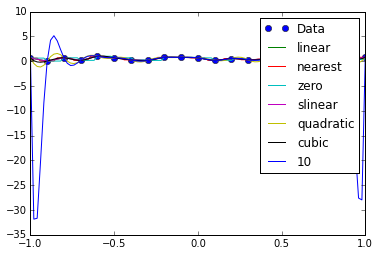
\includegraphics[width=15cm]{1}
 \caption{Captura de pantalla mostrando las diferentes condiciones iniciales para cada animación de péndulo \cite{W}.}
\end{figure}

Basándonos en el tutorial propuesto por Jake Vanderplas \cite{MAT} y un ejemplo de animación de matplotlib \cite{M}, se anexan los códigos en Python para ambas animaciones: el espacio fase y el péndulo simple.

\subsection*{Programa: Animación del espacio fase de un péndulo simple, y de su movimiento}

{\color{RoyalPurple}\begin{verbatim}
from numpy import sin, cos
import numpy as np
import matplotlib.pyplot as plt
import scipy.integrate as integrate
import matplotlib.animation as an
from matplotlib.lines import Line2D
from scipy.integrate import odeint

class DoublePendulum:
    def __init__(self,
                 init_state = [0, 0, 0, 0],
                 L1 = 1.0,  # Longitud del pendulo 1
                 L2 = 0.0,  # Longitud del pendulo 2
                 M1 = 1.0,  # Masa del pendulo 1
                 M2 = 1.0,  # Masa del pendulo 2
                 G = 9.8,   # Aceleracion por la gravedad
                 origin=(0, 0)): 
        self.init_state = np.asarray(init_state, dtype='float')
        self.params = (L1, L2, M1, M2, G)
        self.origin = origin
        self.time_elapsed = 0

        self.state = self.init_state * np.pi / 180.
    
    def position(self):
        (L1, L2, M1, M2, G) = self.params

        x = np.cumsum([self.origin[0],
                       L1 * sin(self.state[0]),
                       L2 * sin(self.state[2])])
        y = np.cumsum([self.origin[1],
                       -L1 * cos(self.state[0]),
                       -L2 * cos(self.state[2])])
        return (x, y)

    def energy(self):
        (L1, L2, M1, M2, G) = self.params

        x = np.cumsum([L1 * sin(self.state[0]),
                       L2 * sin(self.state[2])])
        y = np.cumsum([-L1 * cos(self.state[0]),
                       -L2 * cos(self.state[2])])
        vx = np.cumsum([L1 * self.state[1] * cos(self.state[0]),
                        L2 * self.state[3] * cos(self.state[2])])
        vy = np.cumsum([L1 * self.state[1] * sin(self.state[0]),
                        L2 * self.state[3] * sin(self.state[2])])

        U = G * (M1 * y[0] + M2 * y[1])
        K = 0.5 * (M1 * np.dot(vx, vx) + M2 * np.dot(vy, vy))

        return U + K

    def dstate_dt(self, state, t):
        (M1, M2, L1, L2, G) = self.params

        dydx = np.zeros_like(state)
        dydx[0] = state[1]
        dydx[2] = state[3]

        cos_delta = cos(state[2] - state[0])
        sin_delta = sin(state[2] - state[0])

        den1 = (M1 + M2) * L1 - M2 * L1 * cos_delta * cos_delta
        dydx[1] = (M2 * L1 * state[1] * state[1] * sin_delta * cos_delta
                   + M2 * G * sin(state[2]) * cos_delta
                   + M2 * L2 * state[3] * state[3] * sin_delta
                   - (M1 + M2) * G * sin(state[0])) / den1

        den2 = (L2 / L1) * den1
        dydx[3] = (-M2 * L2 * state[3] * state[3] * sin_delta * cos_delta
                   + (M1 + M2) * G * sin(state[0]) * cos_delta
                   - (M1 + M2) * L1 * state[1] * state[1] * sin_delta
                   - (M1 + M2) * G * sin(state[2])) / den2
        
        return dydx

    def step(self, dt):
        self.state = integrate.odeint(self.dstate_dt, self.state, [0, dt])[1]
        self.time_elapsed += dt

#-----------------------
#CI para el pendulo
theta0= 20
v0= 0
pendulum = DoublePendulum([theta0, v0, 0.0, 0.0])

#-----------------------
#CI para el espacio fase
g = 9.81 #valor de g
l = 1.0 #longitud
b = 0.0 #no friccion
c = g/l

X_f1 =np.array([(theta0/180.0)*np.pi,(v0/180.0)*np.pi])
t = np.linspace(0,50,500)

#ED del pendulo
def p (y, t, b, c):
    theta, omega = y
    dy_dt = [omega,-b*omega -c*np.sin(theta)]
    return dy_dt

#Trayectoria
y0 = X_f1                       
X = odeint(p, y0, t, args=(b,c))         

#-----------------------
#Animacion del pendulo
dt = 1./60.
fig = plt.figure()
ax = fig.add_subplot(111, aspect='equal', autoscale_on=False,
                     xlim=(-2, 2), ylim=(-2, 2))
ax.grid()

line, = ax.plot([], [], 'o-', lw=2, color='m')
time_text = ax.text(0.02, 0.95, '', transform=ax.transAxes)
energy_text = ax.text(0.02, 0.90, '', transform=ax.transAxes)

def init():
    #iniciando animacion
    line.set_data([], [])
    time_text.set_text('')
    energy_text.set_text('')
    return line, time_text, energy_text

def animate(i):
    #animar las fotitos
    global pendulum, dt
    pendulum.step(dt)
    line.set_data(*pendulum.position())
    return line, time_text, energy_text

from time import time
t0 = time()
animate(0)
t1 = time()
interval = 1000 * dt - (t1 - t0)

ani = an.FuncAnimation(fig, animate, frames=300,
                              interval=interval, blit=True, init_func=init)
plt.show()

#-----------------------
#Animacion del espacio fase
class SubplotAnimation(an.TimedAnimation):
    def __init__(self):
        fig = plt.figure()
        ax1 = fig.add_subplot(1, 1, 1)
       
        self.t = np.linspace(0, 80, 400)
        self.x = X[:,0]
        self.y = X[:,1]

        self.line1 = Line2D([], [], color='m')
        self.line1a = Line2D([], [], color='g', linewidth=2)
        self.line1e = Line2D(
            [], [], color='g', marker='o', markeredgecolor='r')
        ax1.add_line(self.line1)
        ax1.add_line(self.line1a)
        ax1.add_line(self.line1e)
        ax1.set_xlim(-2, 2)
        ax1.set_ylim(-2, 2)
        ax1.grid()
        ax1.set_aspect('equal', 'datalim')

        an.TimedAnimation.__init__(self, fig, interval=50, blit=True)

    def _draw_frame(self, framedata):
        i = framedata
        head = i - 1
        head_slice = (self.t > self.t[i] - 1.0) & (self.t < self.t[i])

        self.line1.set_data(self.x[:i], self.y[:i])
        self.line1a.set_data(self.x[head_slice], self.y[head_slice])
        self.line1e.set_data(self.x[head], self.y[head])

    def new_frame_seq(self):
        return iter(range(self.t.size))

    def _init_draw(self):
        lines = [self.line1, self.line1a, self.line1e]
        for l in lines:
            l.set_data([], [])

ani = SubplotAnimation()
plt.show()

#Corri el programa en la terminal para mostrar las animaciones directamente
\end{verbatim}}

En la presente carpeta se encuentran las animaciones en formato mp4 de cada caso. Las miniaturas para cada caso se presentan en la figura 2 a continuación.

\subsection*{Gráficas obtenidas}

\begin{figure}[H]
    \centering
    \begin{subfigure}[b]{0.4\textwidth}
    \centering
        \includegraphics[width=7cm]{0}
        \caption{Péndulo}
    \end{subfigure}
    ~ 
    \begin{subfigure}[b]{0.4\textwidth}
    \centering
        \includegraphics[width=7cm]{f0}
        \caption{Espacio fase.}
    \end{subfigure}
    \caption{$\theta_0=0 \quad v_0=0$.}
\end{figure}

\begin{figure}[H]
    \centering
    \begin{subfigure}[b]{0.4\textwidth}
    \centering
        \includegraphics[width=7cm]{0}
        \caption{Péndulo}
    \end{subfigure}
    ~ 
    \begin{subfigure}[b]{0.4\textwidth}
    \centering
        \includegraphics[width=7cm]{f0}
        \caption{Espacio fase.}
    \end{subfigure}
    \caption{$\theta_0=0 \quad v_0=0$.}
\end{figure}

\begin{figure}[H]
    \centering
    \begin{subfigure}[b]{0.4\textwidth}
    \centering
        \includegraphics[width=7cm]{45}
        \caption{Péndulo}
    \end{subfigure}
    ~ 
    \begin{subfigure}[b]{0.4\textwidth}
    \centering
        \includegraphics[width=7cm]{f45}
        \caption{Espacio fase.}
    \end{subfigure}
    \caption{$\theta_0=45 \quad v_0=0$.}
\end{figure}

\begin{figure}[H]
    \centering
    \begin{subfigure}[b]{0.4\textwidth}
    \centering
        \includegraphics[width=7cm]{90}
        \caption{Péndulo}
    \end{subfigure}
    ~ 
    \begin{subfigure}[b]{0.4\textwidth}
    \centering
        \includegraphics[width=7cm]{f90}
        \caption{Espacio fase.}
    \end{subfigure}
    \caption{$\theta_0=90 \quad v_0=0$.}
\end{figure}

\begin{figure}[H]
    \centering
    \begin{subfigure}[b]{0.4\textwidth}
    \centering
        \includegraphics[width=7cm]{135}
        \caption{Péndulo}
    \end{subfigure}
    ~ 
    \begin{subfigure}[b]{0.4\textwidth}
    \centering
        \includegraphics[width=7cm]{f135}
        \caption{Espacio fase.}
    \end{subfigure}
    \caption{$\theta_0=135 \quad v_0=0$.}
\end{figure}

\begin{figure}[H]
    \centering
    \begin{subfigure}[b]{0.4\textwidth}
    \centering
        \includegraphics[width=7cm]{170}
        \caption{Péndulo}
    \end{subfigure}
    ~ 
    \begin{subfigure}[b]{0.4\textwidth}
    \centering
        \includegraphics[width=7cm]{f170}
        \caption{Espacio fase.}
    \end{subfigure}
    \caption{$\theta_0=170 \quad v_0=0$.}
\end{figure}

\begin{figure}[H]
    \centering
    \begin{subfigure}[b]{0.4\textwidth}
    \centering
        \includegraphics[width=7cm]{180}
        \caption{Péndulo}
    \end{subfigure}
    ~ 
    \begin{subfigure}[b]{0.4\textwidth}
    \centering
        \includegraphics[width=7cm]{f180}
        \caption{Espacio fase.}
    \end{subfigure}
    \caption{$\theta_0=180 \quad v_0=0$.}
\end{figure}

\begin{figure}[H]
    \centering
    \begin{subfigure}[b]{0.4\textwidth}
    \centering
        \includegraphics[width=7cm]{e1}
        \caption{Péndulo}
    \end{subfigure}
    ~ 
    \begin{subfigure}[b]{0.4\textwidth}
    \centering
        \includegraphics[width=7cm]{fe1}
        \caption{Espacio fase.}
    \end{subfigure}
    \caption{$\theta_0=181 \quad v_0=5$.}
\end{figure}

\begin{figure}[H]
    \centering
    \begin{subfigure}[b]{0.4\textwidth}
    \centering
        \includegraphics[width=7cm]{e2}
        \caption{Péndulo}
    \end{subfigure}
    ~ 
    \begin{subfigure}[b]{0.4\textwidth}
    \centering
        \includegraphics[width=7cm]{fe2}
        \caption{Espacio fase.}
    \end{subfigure}
    \caption{$\theta_0=182 \quad v_0=20$.}
\end{figure}

\begin{thebibliography}{6}

\bibitem{W}
Wikipedia.
\emph{Pendulum}. Recuperado en mayo de 2016 de \url{https://en.wikipedia.org/wiki/Pendulum_(mathematics)#Examples}

\bibitem{MAT}
Vanderplas, J.
\emph{Matplotlib Animation Tutorial}. Recuperado en mayo de 2016 de \url{https://jakevdp.github.io/blog/2012/08/18/matplotlib-animation-tutorial/}

\bibitem{M}
Matplotlib.
\emph{Animation example code: Double pendulum animated}. Recuperado en mayo de 2016 de \url{http://matplotlib.org/examples/animation/double_pendulum_animated.html}

\bibitem{FC}
Lizárraga, C.
\emph{Actividad 10 (2016-1)}. Recuperado en mayo de 2016 de \url{http://computacional1.pbworks.com/w/page/107247876/Actividad\%2010\%20(2016-1)}

\end{thebibliography}

\end{document}

